%%%%% this line is 80 chars wide, please don't make longer lines %%%%%%%%%%%%%%%
The "Auditory Neuroscience" book\cite{AuditoryNeuroscience} tells us in the 
chapter two what is important for us here to know. 

Like written before, the auditory system has (generally air) pressure as input, 
and spike trains as output. We will go through the parts of the ear, with help 
of the next image, which comes from the page 52 of the submentioned book. 

We have first the external ear. There the pressure signals come through the ear 
canal and make the eardrum vibrate. This takes us to the medium ear. 
The vibration is propagated throughout it by three ossicles : malleus, incus 
and stapes. The farthest part from the external ear of the stapes touches the 
boundary of the cochlea, on the oval window, in the inner ear, and makes vibrate
 the liquid in it. 
In the cochlea we have the interface between this mechanical vibration 
and the neural signal that will go through the auditory nerve 
(VII nerve on the image).

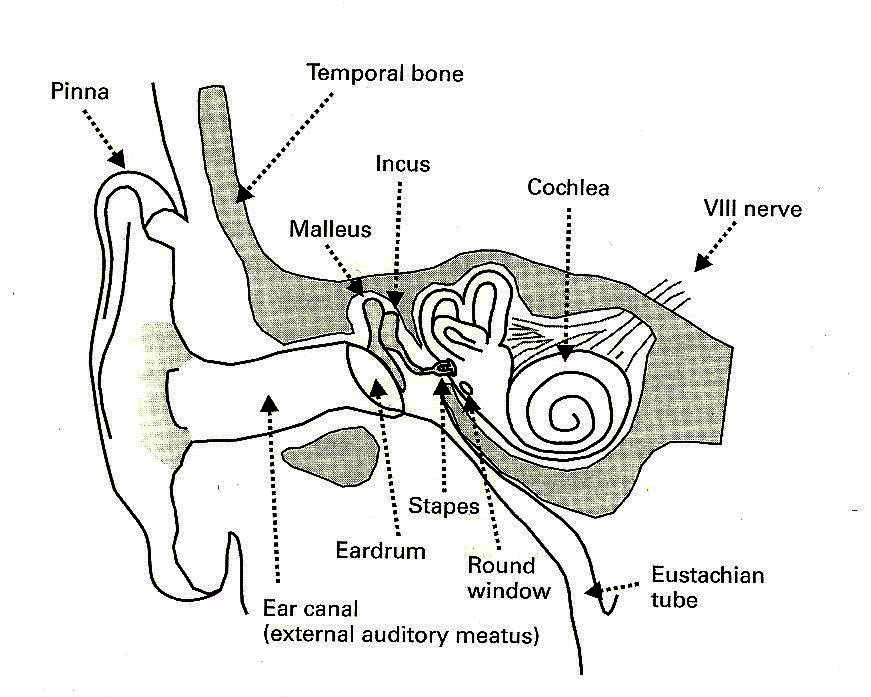
\includegraphics[width=0.4\textwidth]{images/ear-aud52-level.jpg}

We will interest ourselves after more in this interface. But first we should see 
more on the vibration of the cochlea. The cochlea has two main compartments, 
that are one above the other and separated 
throughout the tube except at the far end of it by a membrane that is called 
the basilar membrane, as you can see on the image 
(from page 55 of the "Auditory Neuroscience" book).

%\includegraphics[width=0.4\textwidth]{images/55}

A vibration that comes will try to propagate through the basilar membrane from 
the upper compartment to the other. When doing that, it will not make all 
the parts of the basilar membrane vibrate at the same intensity. 
In fact, the cochlea is like a "biological Fourier analyzer" according to the book. 
The frequency content of vibrations is decomposed and each frequency has its 
"favorite" place in the cochlear coiled tube that it makes vibrate particularily. 
The part of the basilar membrane that is the first we can see vibrating, 
when we gradually put on the volume of a pure tone of frequency f, is said to be of 
"characteristic frequency" f. Near the oval window, the characteristic 
frequencies are high, and as we go to the tip of the tube, 
the characteristic frequency becomes lower.

Throughout the cochlear tube, we have the organ of Corti, which is the interface
about which an allusion was made above in the text. We will use another image, 
which comes this time from page 65 of the book.

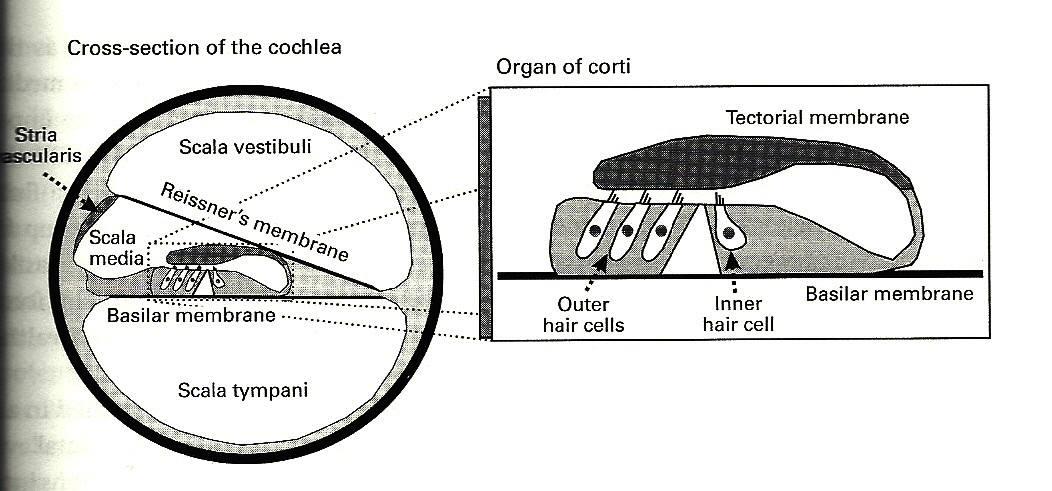
\includegraphics[width=0.4\textwidth]{images/corti-aud65-level.jpg} %do a better one : perhaps two parts ?

The upper compartment of the cochlea is in fact in two parts separated by a membrane.
In the scala media, where we find the organ of Corti, has a higher 
concentration of potassium cations. 

%image p65 